\documentclass[journal,10pt,twocolumn]{article}
\usepackage{graphicx, float}
\usepackage[margin=0.5in]{geometry}
\usepackage{amsmath, bm}
\usepackage{array}
\usepackage{booktabs}

\providecommand{\norm}[1]{\left\lVert#1\right\rVert}
\let\vec\mathbf
\newcommand{\myvec}[1]{\ensuremath{\begin{pmatrix}#1\end{pmatrix}}}
\newcommand{\mydet}[1]{\ensuremath{\begin{vmatrix}#1\end{vmatrix}}}

\title{\textbf{Conics Assignment}}
\author{Pallavarapu Sravan kumar}
\date{October 2022}

\begin{document}

\maketitle
\paragraph{\textit{\large Problem Statement}:Through the vertex O of parabola y$^2$=4x, chords OP and OQ are drawn at right angles to one another show that for all positions of P,PQ cuts the axis of the parabola a fixed point. Also find the locus of the middle point of PQ}
\section*{\large Solution}
\begin{figure}[H]
\centering
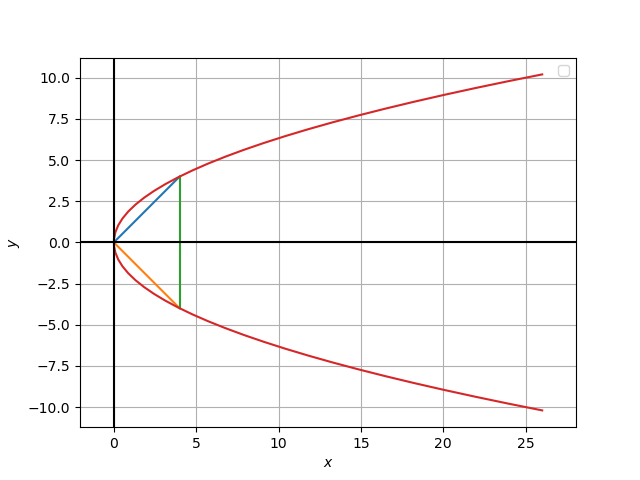
\includegraphics[width=1\columnwidth]{conic.png}
\caption{The intersection of PQ with x-axis  is (4,0)}
\end{figure}

\section*{\large Construction}

\begin{table}[htbp]
 \begin{center}
    \begin{tabular}{|l|c|c|c|c|c|c} \hline \textbf{Symbol}
  & \textbf{value} & \textbf{Description} \\
 \hline
V &\myvec{0\\0} & Vertex of parabola\\ \hline
F&\myvec{-2\\0} & focus of parabola\\ \hline
n &\myvec{1\\0}   & normal of directrix\\ \hline

 
\end{tabular}   
\end{center}
\caption{\label{table:dummytable} }
\end{table}



\section*{Proof:}


The given equation of parabola $y^2 = 4x$ and vertex $\vec{O}=\myvec{0\\0}$
\begin{align}
    \label{eq:conic_quad_form}
    \vec{x}^{\top}\vec{V}\vec{x}+2\vec{u}^{\top}\vec{x}+f=0
    \end{align}
the parametric coordinates of the parabola are P and Q 
\begin{equation*}
 \vec{P} = \myvec{at_1^2\\2at_1} ,\hspace{2mm}\vec{Q} = \myvec{at_2^2\\2at_2}
\end{equation*}
from above parabola equation a=1\\
let us consider $t_1=2 $ and $t_2=-2$,then
\begin{align*}
\vec{P = \myvec{4\\4} ,\hspace{2mm} Q = \myvec{4\\-4}}
\end{align*}
the line equatin of OP and OQ is 
\begin{align*}
\vec{A = OP = O-P}\\
\vec{B = OQ = Q-O}
\end{align*}
Then,
\begin{align*}
\vec{A} = \myvec{-4\\-4}\\
\vspace{1mm}
\vec{B} = \myvec{4\\-4}
\end{align*}
given that $\vec{OP \perp OQ}$to find that 
\begin{align*}
\theta =cos^{-1}\vec{(\frac{A^TB}{\|A\|\|B\|})}
\end{align*}
on solving we get $\theta$ = 90. 
Therefore, $ \vec{A}$ and $\vec{B} $ are $\perp $ satisfy the given condition\\
the equation of PQ is 
\begin{align*}
 \vec{C = PQ = P-Q}
\end{align*}
the intersection of $\vec{PQ}$ line and X-axis gives the fixed point 
\begin{align*}
\vec{X = \myvec{4\\0}}
\end{align*}
the mid point of $\vec{P}$ and $\vec{Q}$ 
\begin{align*}
\vec{R = \frac{P+Q}{2}}\\
\vec{R = \myvec{4\\0}}
\end{align*}
\end{document}